\documentclass[a4paper, 12pt]{article}

\usepackage{hyperref}
\usepackage[warn]{mathtext}
\usepackage[utf8]{inputenc}
\usepackage[T2A]{fontenc}
\usepackage[english,russian]{babel}
\usepackage{multirow}
\usepackage{amsmath,amsfonts,amssymb,amsthm,mathtools}
\usepackage{indentfirst}
\DeclareSymbolFont{T2Aletters}{T2A}{cmr}{m}{it}
\usepackage{ gensymb }
\mathtoolsset{showonlyrefs=true}
\usepackage{euscript}
\usepackage{mathrsfs}
\usepackage[left=2cm,right=2cm,top=2cm,bottom=2cm]{geometry}
\usepackage{graphicx}
\usepackage{wrapfig}
\usepackage[rgb]{xcolor}
\hypersetup{
colorlinks=true,
urlcolor=blue
}


\title{Лабораторная работа}
\author{Гисич Арсений Б03-102}
\date{2022}

\begin{document}

	\begin{center}
		{\large МОСКОВСКИЙ ФИЗИКО-ТЕХНИЧЕСКИЙ ИНСТИТУТ (НАЦИОНАЛЬНЫЙ ИССЛЕДОВАТЕЛЬСКИЙ УНИВЕРСИТЕТ)}
	\end{center}
	\vspace{5 cm}
	{\Large
		\begin{center}
			{\bf Лабораторная работа 3.4.2}\\[0.2 cm]
			Закон Кюри-Вейсса
		\end{center}
	}
	\vspace{4 cm}
	\begin{flushright}
		{\Large Выполнил: \\
			\vspace{0.2 cm}
			Гисич Арсений \\
			\vspace{0.2 cm}
			Б03-102 \\}
	\end{flushright}
	\vspace{9 cm}
	\begin{center}
		Долгопрудный\\[0.1 cm]
		2022
	\end{center}
\thispagestyle{empty}

\section{Аннотация}

В данной работе проводится исследование зависимости магнитной восприимчивости гадолиния, который является ферромагнетиком, от температуры. Исследование проведено для температур от 14 до 40 \textcelsius. На основании этой зависимости вычисляется точка Кюри гадолиния.

\section{Теоретические сведения}

Вещества с отличными от нуля атомными магнитными моментами обладают парамагнитными свойствами. Внешнее магнитное поле ориентирует магнитные моменты, которые в отсутствие поля располагались в пространстве хаотическим образом. Однако при $T \rightarrow 0$ тепловое движение всё меньше препятствует магнитным моментам атомов ориентироваться в одном направлении при сколь угодно слабом внешнем поле. В ферромагнетиках --- под влиянием обменных сил --- это происходит при понижении температуры не до абсолютного нуля, а до температуры Кюри $\Theta_K$. Оказывается, что у ферромагнетиков магнитная восприимчивость должна удовлетворять закону Кюри-Вейсса:
\begin{equation} \label{eq:Kuri-Veicca}
	\chi \propto \frac{1}{T-\Theta_p},
\end{equation}
где $\Theta_p$ --- температура, близкая к температуре Кюри, так как при $T \approx \Theta_K$ формула~\eqref{eq:Kuri-Veicca} недостаточна точна.

\section{Методика измерений}

Схема установки для проверки справедливости закона Кюри-Вейсса показана на рис.~\ref{ris1}. Исследуемый ферромагнитный образец (гадолиний) расположен внутри пустотелой катушки самоиндукции, которая служит индуктивностью колебательного контура, входящего в состав $L C$ -автогенератора.

\begin{figure}[h!]
\begin{center}
    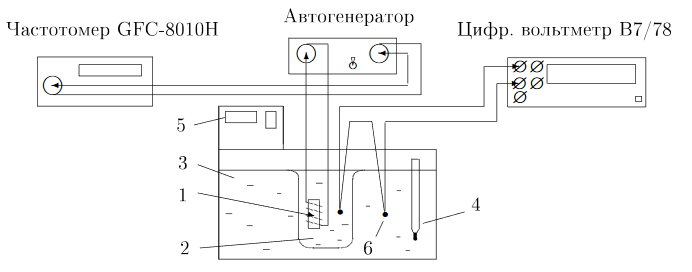
\includegraphics[scale=0.8]{1.png}
\end{center}
\caption{Схема экспериментальной установки}
\label{ris1}
\end{figure}

Гадолиний является хорошим проводником электрического тока, a paбoчая частота генератора достаточно велика $(\sim 50$ кГц $),$ поэтому для уменьшения вихревых токов образец изготовлен из мелких кусочков размером $\sim 0,5$ мм. Катушка 1 с образцом помещена в стеклянный сосуд 2, залитый трансформаторным маслом. Масло предохраняет образец от окисления и способствует ухудшению электрического контакта между отдельными частичками образца. Кроме того, оно улучшает тепловой контакт между образцом и термостатируемой (рабочей) жидкостью 3 в термостате. Ртутный термометр 4 используется для приближённой оценки температуры. Температура образца регулируется с помощью термостата 5.

Магнитная восприимчивость образца $\chi$ определяется по изменению самоиндукции катушки. Обозначив через $L$ самоиндукцию катушки с образцом и через $L_0$ -- её самоиндукцию в отсутствие образца, получим
\begin{equation*}
	(L-L_0)\propto \chi.
\end{equation*}
При изменении самоиндукции образца меняется период колебаний автогенератора:
\begin{equation*}
	\tau = 2\pi \sqrt{LC},
\end{equation*}
где $C$ --- ёмкость контура автогенератора. Период колебаний в отсутствие образца определяется самоиндукцией пустой катушки:
\begin{equation*}
	\tau_0 = 2\pi \sqrt{L_0C}.
\end{equation*}

Итак, закон Кюри-Вейсса справедлив, если выполнено соотношение:
\begin{equation}
	\frac{1}{\chi} \propto (T-\Theta_p) \propto \frac{1}{\tau^2-\tau_0^2}.
\end{equation}

Измерения проводятся в интервале температур от 14~\textcelsius\, до 40~\textcelsius.

\section{Используемое оборудование}

\begin{enumerate}
    \item катушка самоиндукции с образцом из гадолиния;
    \item термостат;
    \item частотомер;
    \item цифровой вольтметр;
    \item $LC$-автогенератор;
    \item термопара медь-константан;
\end{enumerate}

\section{Результаты измерений и обработка данных}

Результаты измерений периода колебаний $\tau$, ЭДС термопары $\Delta{U}$ и температуры термостата $T$ представлены в таб.~\ref{tab1}. Период колебаний без образца $\tau_0 = 8,252~мкс$. Температурный коэффициент термопары $k^{-1} = 24~\frac{\celsius}{мВ}$.

\newpage

\begin{table}[h!]
\begin{center}
\begin{tabular}{|c|c|c|c|c|c|}
\hline
$\tau, мкс$ & $\delta_{\tau}, мкс$ & $T, \celsius$ & $\delta_T, \celsius$ & $\Delta{U}, мВ$ & $\delta_{\Delta{U}}, мВ$ \\ \hline
10,068 & 0,001 & 14,04 & 0,01 & -0,012 & 0,001 \\ \hline
9,955 & 0,001 & 16,03 & 0,01 & -0,017 & 0,001 \\ \hline
9,753 & 0,001 & 18,03 & 0,01 & -0,014 & 0,001 \\ \hline
9,433 & 0,001 & 20,03 & 0,01 & -0,015 & 0,001 \\ \hline
9,042 & 0,001 & 22,01 & 0,01 & -0,016 & 0,001 \\ \hline
8,747 & 0,001 & 24,02 & 0,01 & -0,017 & 0,001 \\ \hline
8,609 & 0,001 & 26,01 & 0,01 & -0,017 & 0,001 \\ \hline
8,534 & 0,001 & 28,01 & 0,01 & -0,015 & 0,001 \\ \hline
8,488 & 0,001 & 30,00 & 0,01 & -0,017 & 0,001 \\ \hline
8,453 & 0,001 & 32,00 & 0,01 & -0,017 & 0,001 \\ \hline
8,429 & 0,001 & 34,00 & 0,01 & -0,018 & 0,001 \\ \hline
8,409 & 0,001 & 36,01 & 0,01 & -0,016 & 0,001 \\ \hline
8,395 & 0,001 & 38,00 & 0,01 & -0,016 & 0,001 \\ \hline
8,383 & 0,001 & 40,00 & 0,01 & -0,017 & 0,001 \\ \hline
\end{tabular}
\end{center}
\caption{Результаты измерения зависимости периода колебаний $LC$-генератора от температуры образца}
\label{tab1}
\end{table}

Полученный график зависимости $\frac{1}{\tau^2-\tau_0^2} = f(T)$ представлен на рис.~\ref{ris2}.

\begin{figure}[h!]
\begin{center}
    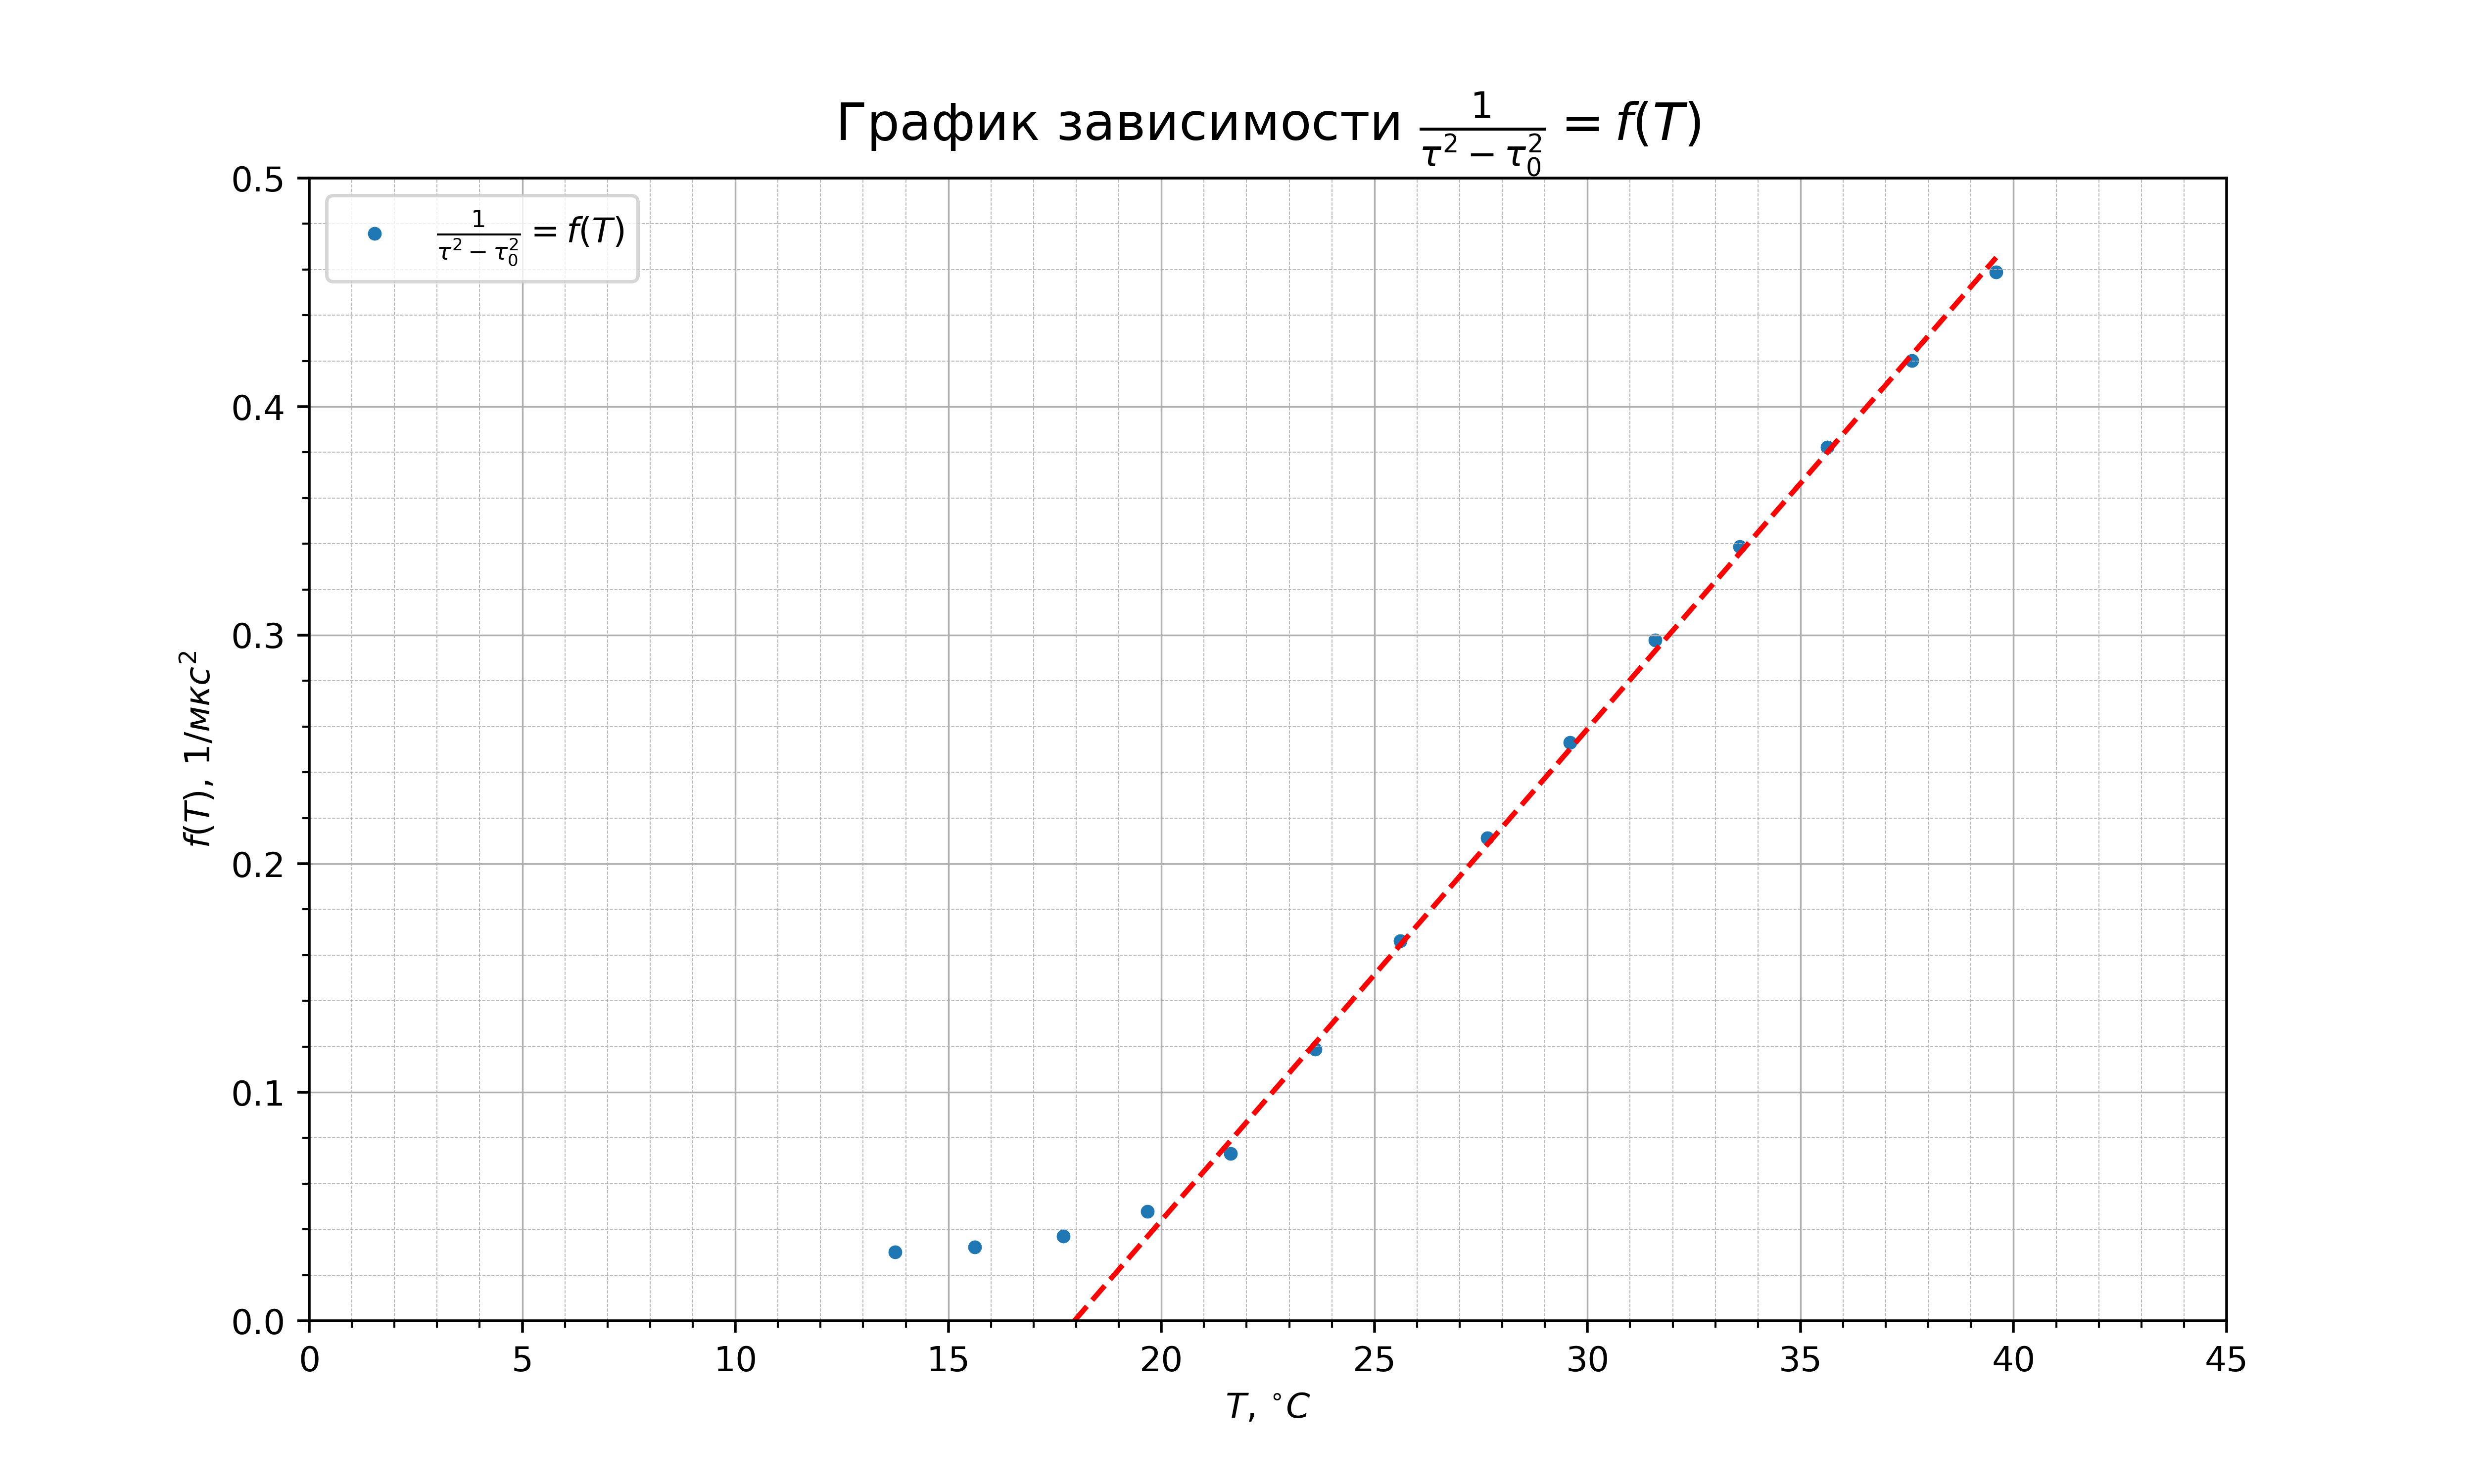
\includegraphics[scale=0.7]{3.4.2_1.png}
\end{center}
\caption{График зависимости $\frac{1}{\tau^2-\tau_0^2}$ от температуры}
\label{ris2}
\end{figure}

Экстраполяция даёт значение парамагнитной точки Кюри $\Theta_p = 17,96\pm0,03~\celsius$. Оценочное значение ферромагнитной точки Кюри --- $\Theta_K = 15\pm2~\celsius$. Эта точка находится приблизительно в том месте, где график выходит на прямую и уходит в 0. В данном случае график выходит на прямую, но не доходит до 0. Вероятно, имеет место систематическая погрешность.


\section{Обсуждение результатов и выводы}

В данной работе была исследована температурная зависимость магнитной восприимчивости гадолиния выше точки Кюри. Также была рассчитана парамагнитная точка Кюри для данного металла.

Полученное значение парамагнитной точки Кюри: $$\boxed{\Theta_p = 17,96\pm0,03~\celsius}$$
Данное значение существенно отличается от табличного (20,2~\textcelsius). Основной вклад в погрешность вносит погрешность определения температуры образца. Расхождение может быть вызвано неравномерным нагревом установки и сосуда с образцом. Как и предполагалось законом Кюри-Вейсса, данная температура выше ферромагнитной точки Кюри, которая равна 16~\textcelsius{}. Также, данное значение согласуется с оценочным, полученным из графика.

\end{document}
